\chapter{Le cadre de mesure}

Le cadre de mesure a été réalisé en bois. Les dimensions ont été choisi afin de limiter au maximum l'encombrement et en concertation avec notre client, M. Singhoff, afin que l'environnement des abeilles ne soit pas perturbé. Sa hauteur maximale a été fixé à 1 cm. Cette taille lui permet de rester à la fois discret une fois monté sur la ruche et de faciliter les actions de l'apiculteur car il aura juste à retirer un seul élément.\\
Cette contrainte nous a conduit à réétudier la conception du cadre pour finalement placer les capteurs entre une couche de bois et une couche de métal ce qui le rendra plus rigide et moins épais qu'entre deux couches de bois.\\
Le cadre a été dessiné sur Catia puis fabriqué grâce à la fraiseuse de l'ENSTA Bretagne en deux parties qui viendront s'emboiter lors du montage.\\

\begin{figure}[h!]
\centering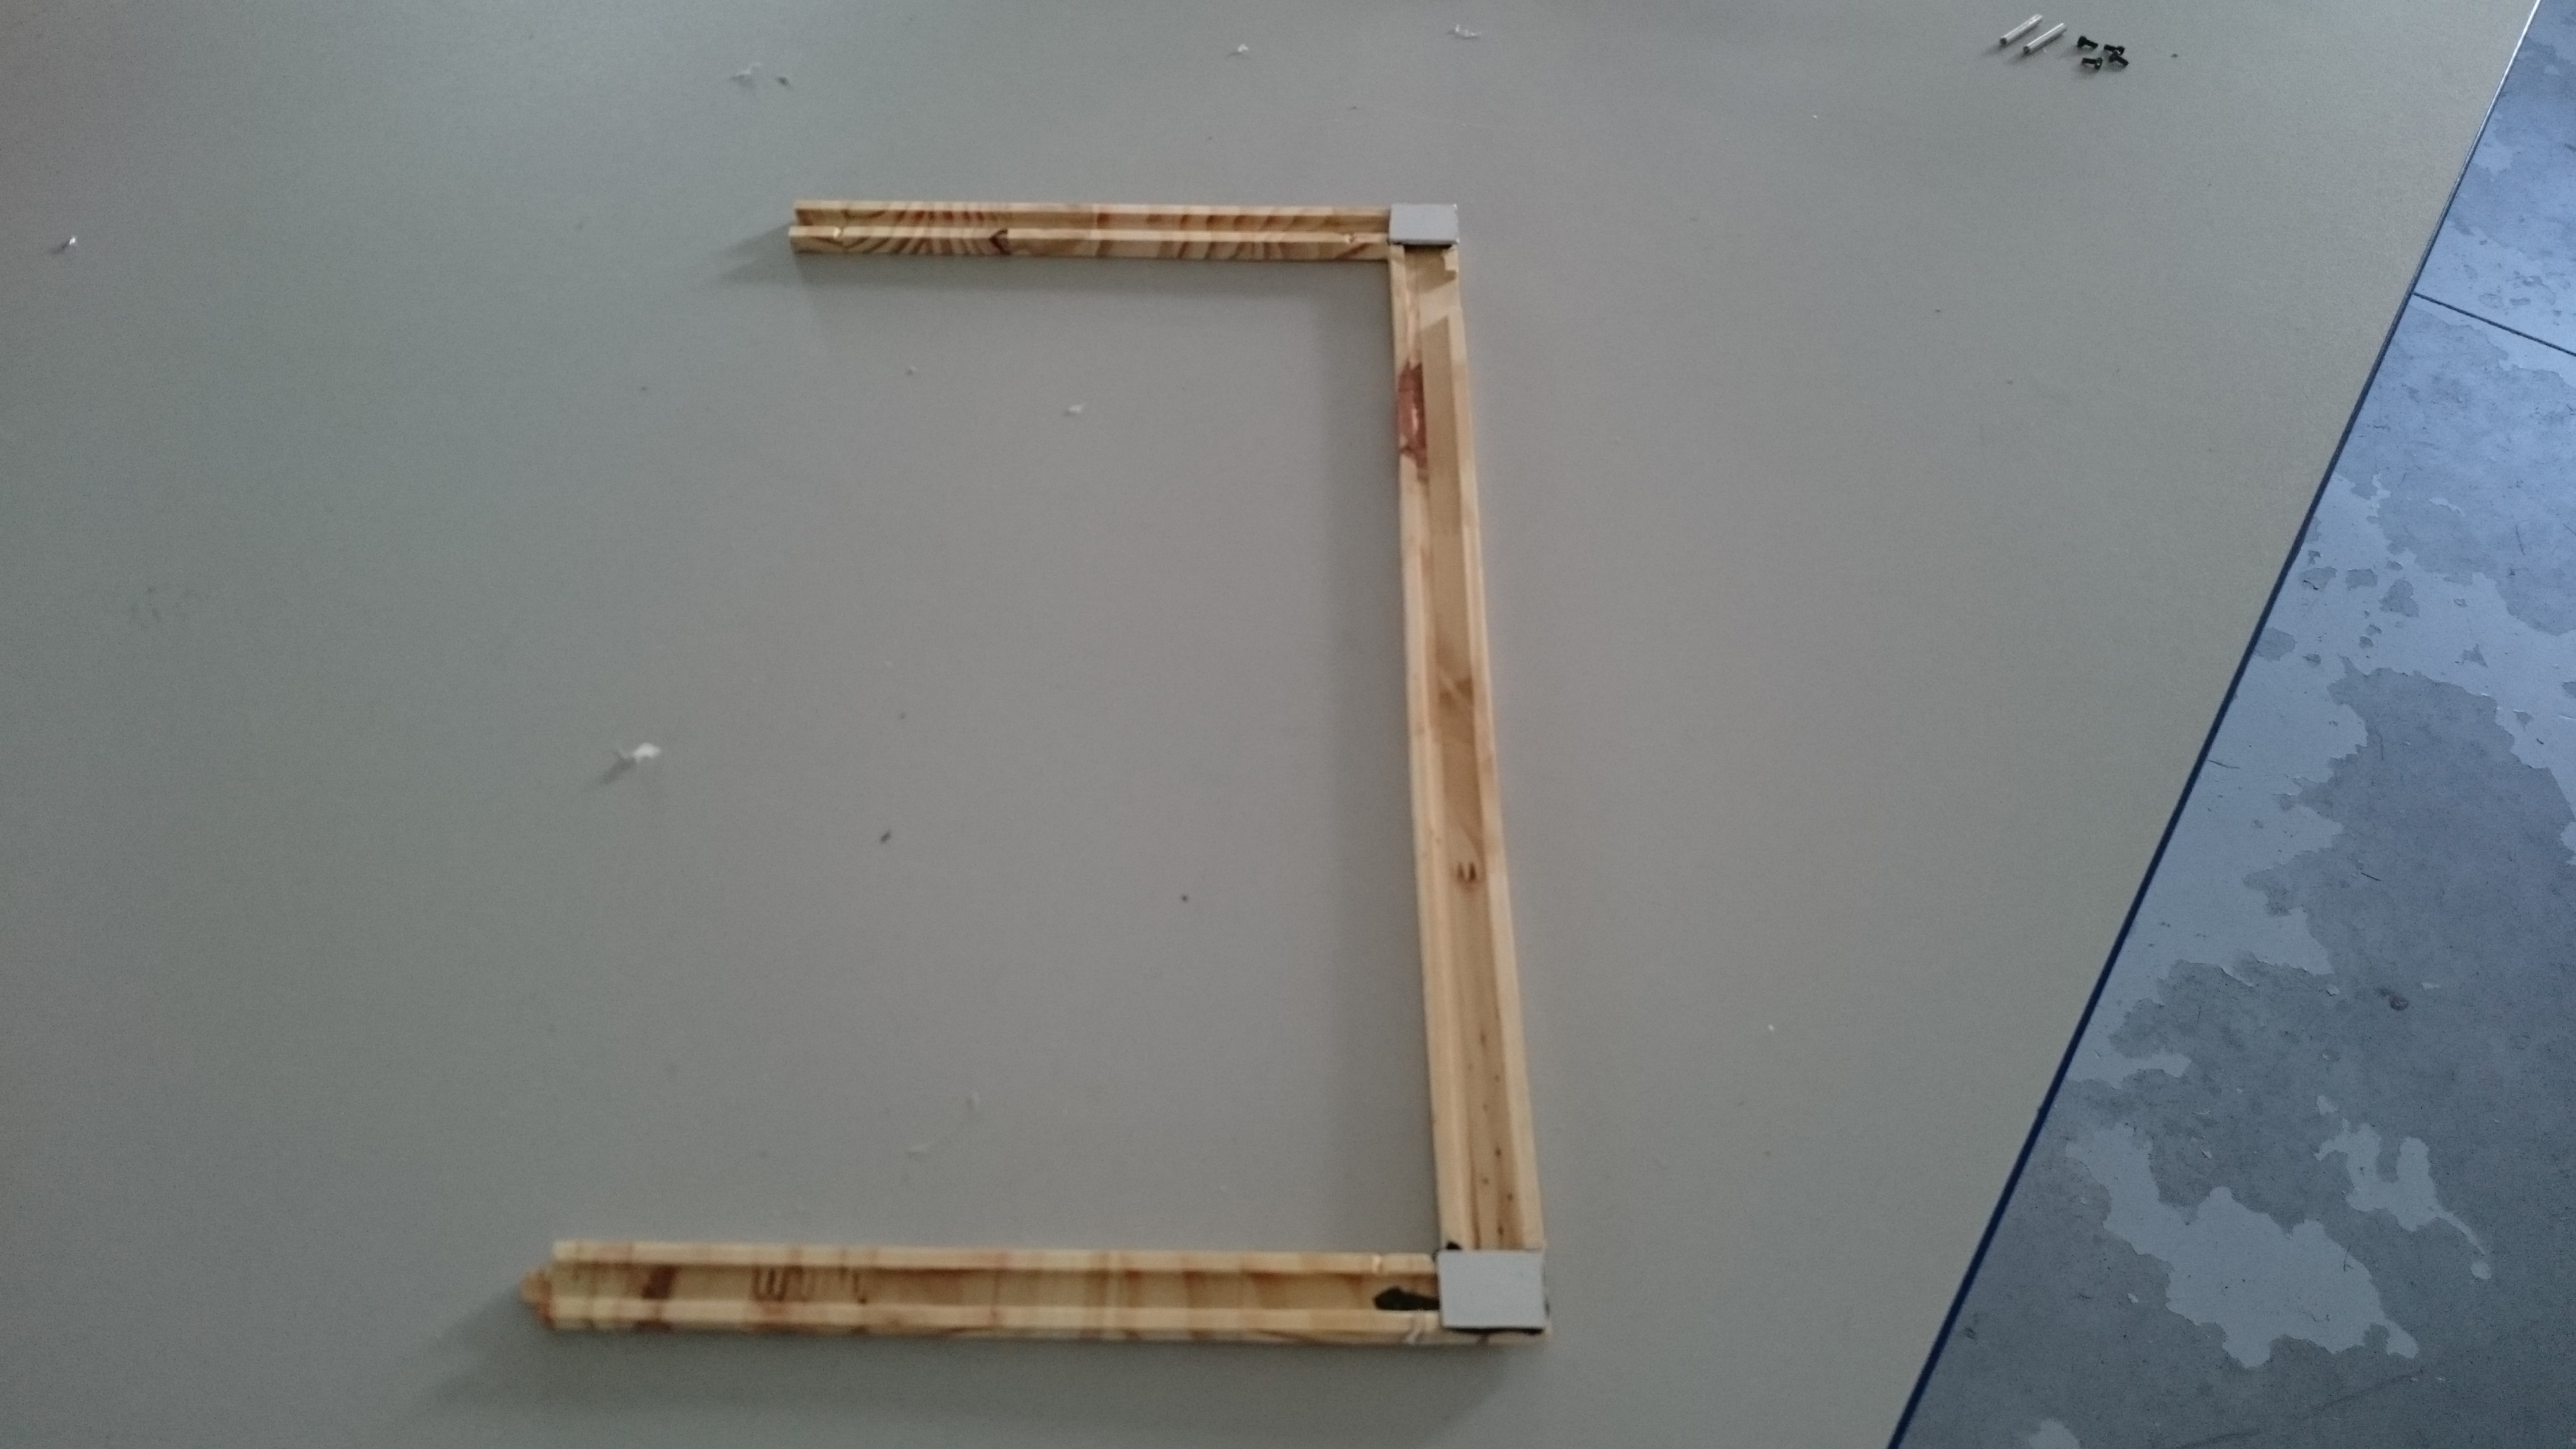
\includegraphics[trim= 0cm 0cm 0cm 0cm,scale=0.08]{cadre.jpg}
\caption{\label{fig:cote1} Schéma d'une des deux parties du cadre de mesure}
\end{figure}

\clearpage

\section{Intégration des capteurs}

Nous avons décidé de positionner 14 capteurs sur notre cadre afin de recueillir 5 paramètres:\\

\indent - 6 thermistances \\
\indent - 4 capteurs de pression \\ 
\indent - 2 tilt \\ 
\indent - 1 capteur de son \\
\indent - 1 capteur d'humidité \\

Ces capteurs ont été disposé comme sur la figure \ref{fig:face} présenté dans le chapitre 5: Architecture physique. Chaque capteur est relié à 2 ou 3 fils pour ceux qui sont déjà installé sur une carte. C'est le cas pour les trois derniers capteurs ci-dessus. Pour les thermistances et les capteurs de pressions, nous les avons monté sur une carte en série avec des résistances de 10 kOhm pour les premiers et 1.8 kOhm pour les second. Le choix d'une résistance faible pour les capteurs de pression nous permet d'avoir une meilleur précision au niveau de la plage de masse qui nous intéresse. Ces capteurs de poids permettrons soit de récupérer le poids de la ruche et ainsi suivre l'évolution de la colonie, soit celle des hausse et donc suivre la miellée.\\

Avant d'être intégrés au cadre, les capteurs ont été testé individuellement. Les capteurs de pression qui permettront de déterminer le poids de la ruche ont notamment dû être étalonnés. Nous avons réalisé cette manipulation dans un des laboratoires de mécanique de l'école. Comme nous pouvons le voir sur la figure \ref{fig:pression}, nous avons placé chaque capteur de pression sur une machine capable d'exercer une gamme prédéfinie de pressions sur la zone de test. Nous avons relevé la réponse du capteur, une tension entre 0 et 5 volts, pour chaque échantillon lors de trois séries de mesures. Ces séries étaient composées d'un ensemble d'échantillons répartis comme suit: 20 valeurs croissantes de force de 0 à 100 Newtons puis 20 valeurs décroissantes de 100 à 0 Newton.

\begin{figure}[h]
\centering
	\subfigure{
		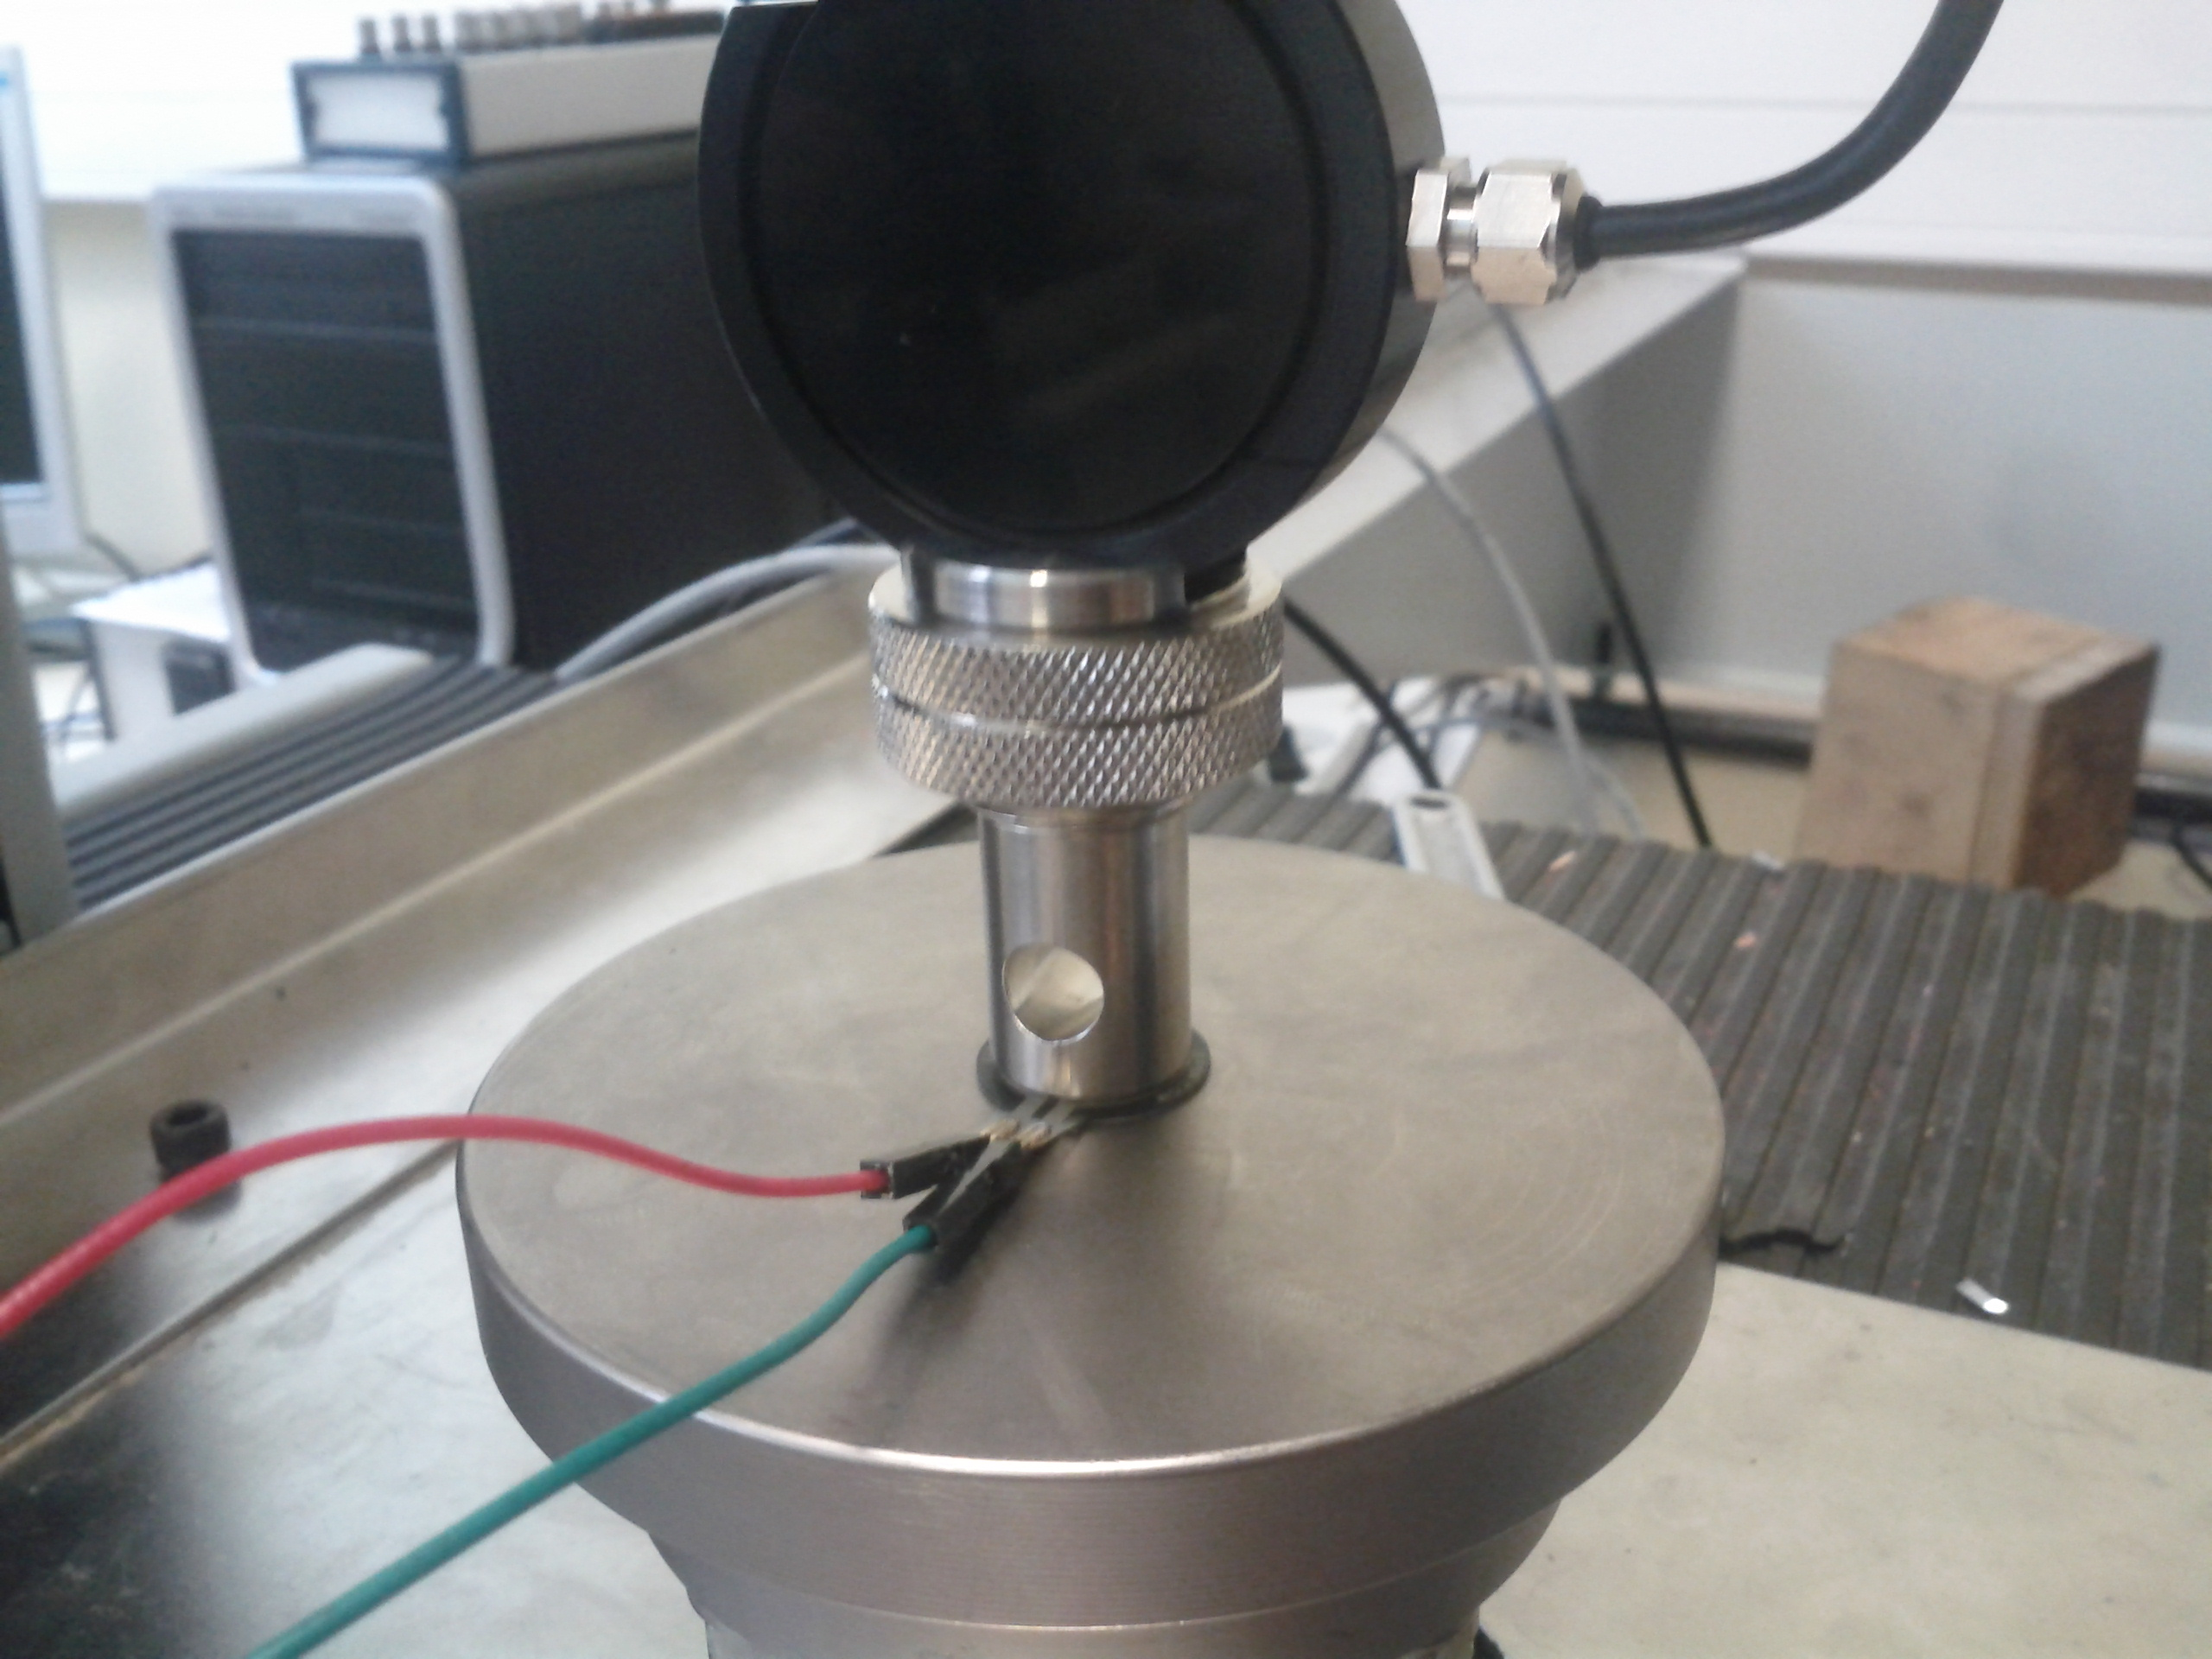
\includegraphics[scale=0.08]{testPression1.jpg}
		}
	\quad
	\subfigure{
		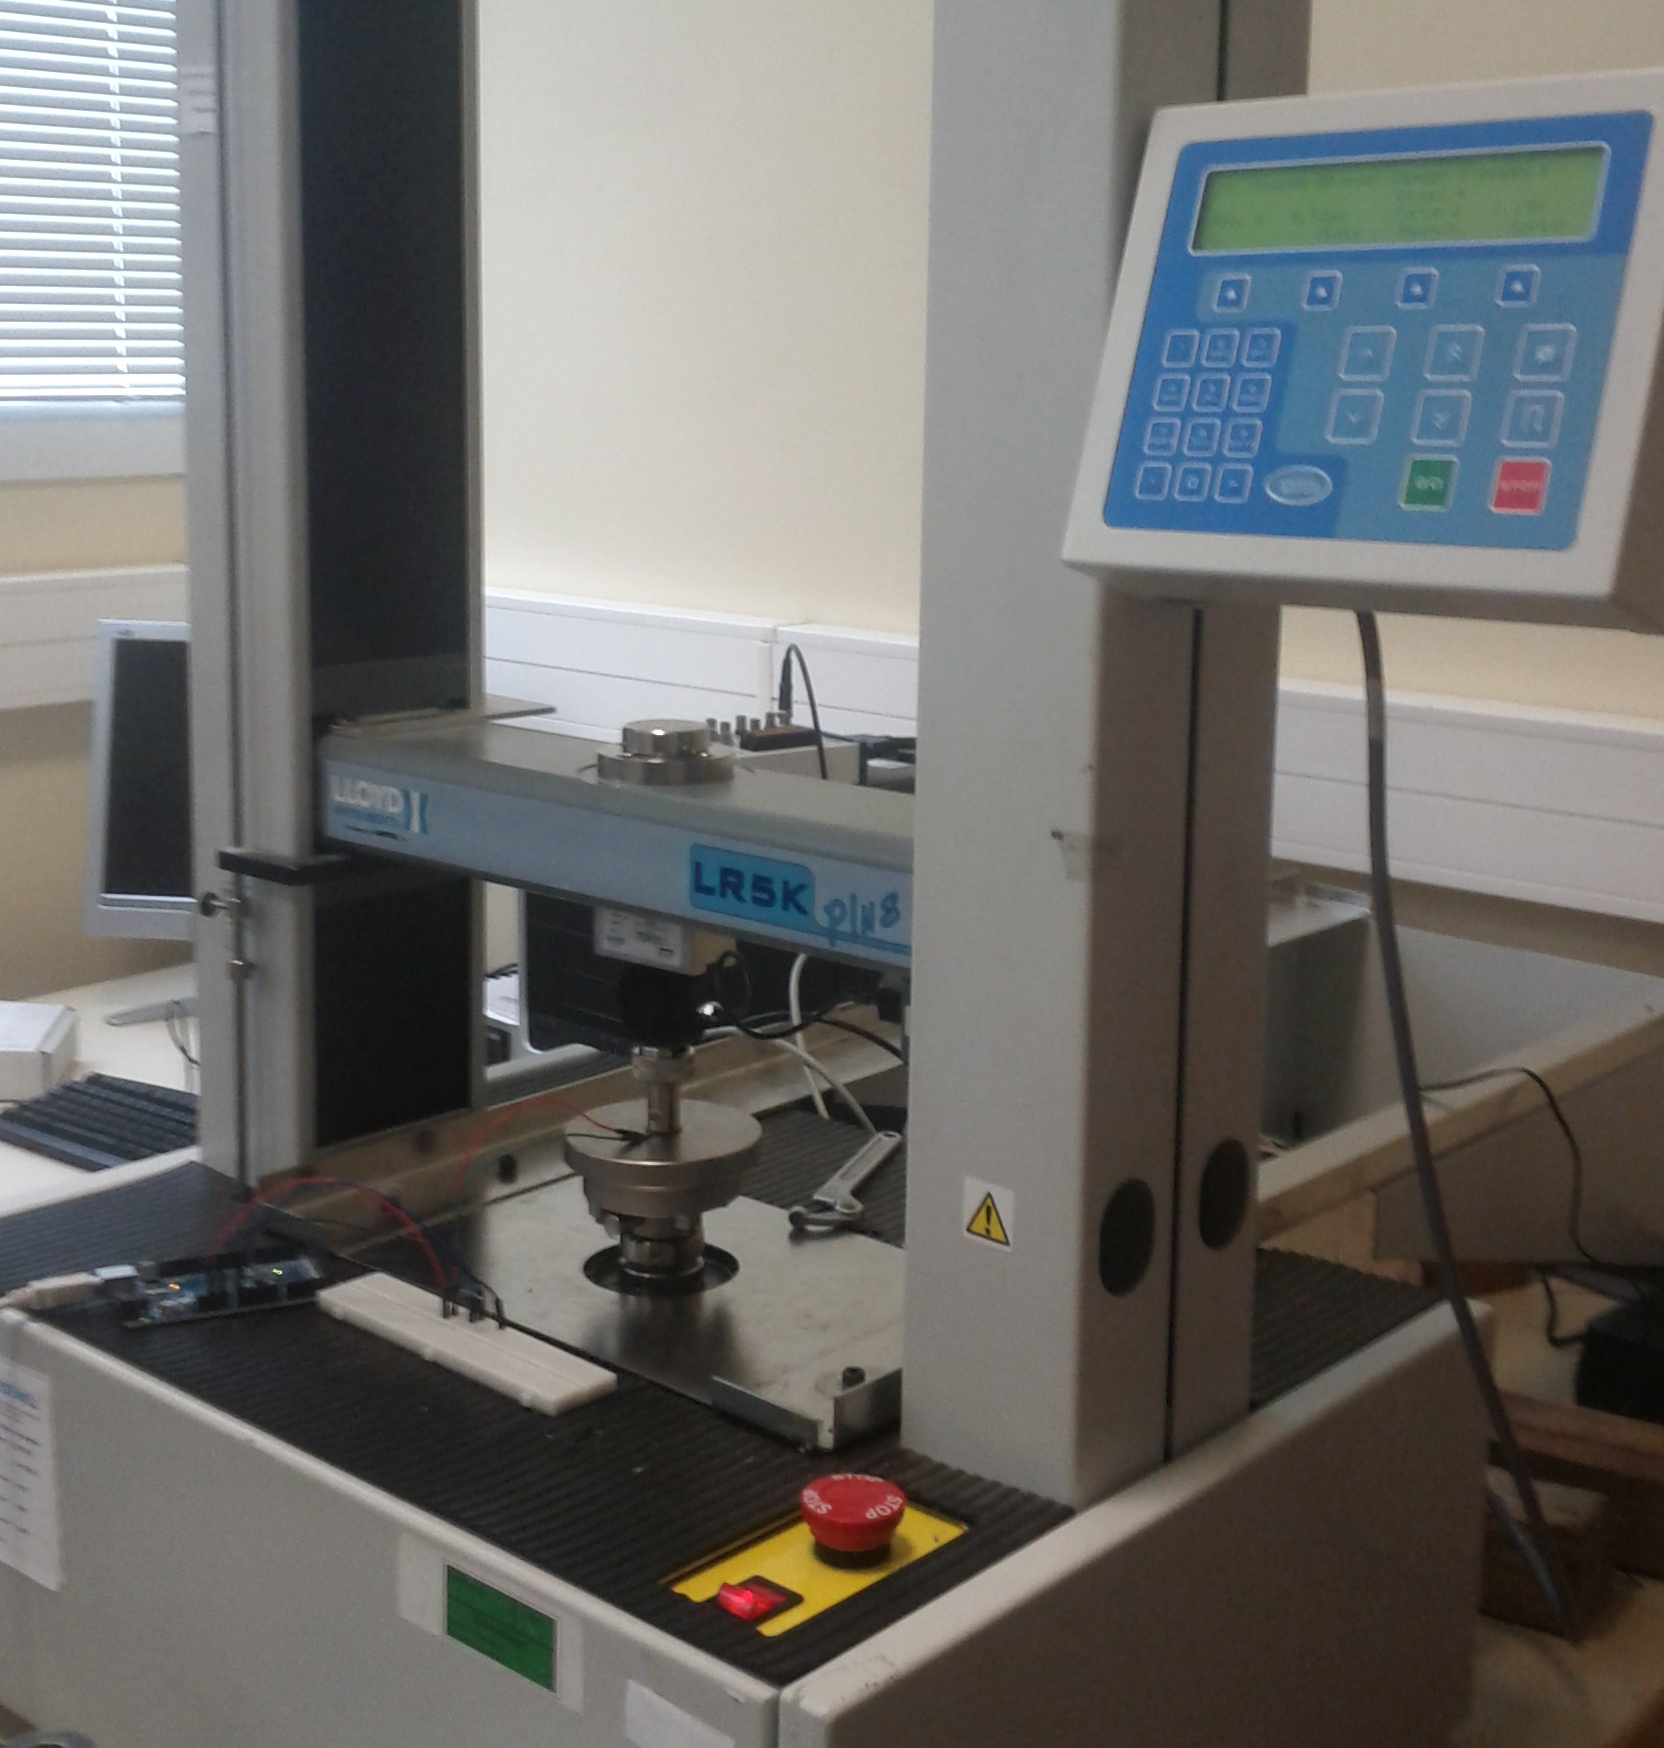
\includegraphics[scale=0.1]{testPression2.jpg}
		}
	\caption{\label{fig:pression} \'Etalonnage des capteurs de pression dans un laboratoire de mécanique de l'ENSTA Bretagne }
\end{figure}


L'ensemble des valeurs obtenues nous a permis de tracer la courbe qui nous donne une mesure de masse en fonction de la tension en sortie du capteur, voir figure \ref{fig:courbe}. Nous avons ensuite obtenu une équation de cette courbe de tendance. L'équation de cette courbe est de type polynomiale de degré 6 et $R²=0.96$. Comme les calculs de conversion ne seront pas effectués par l'Arduino mais par le serveur, la forme de cette équations n'est pas problématique. Nous avons également vérifié que tous les capteurs de pression suivent bien la même loi. Nous avons donc une formule unique de conversion de la tension de sortie en masse appliquée.

\begin{figure}[!h]
\centering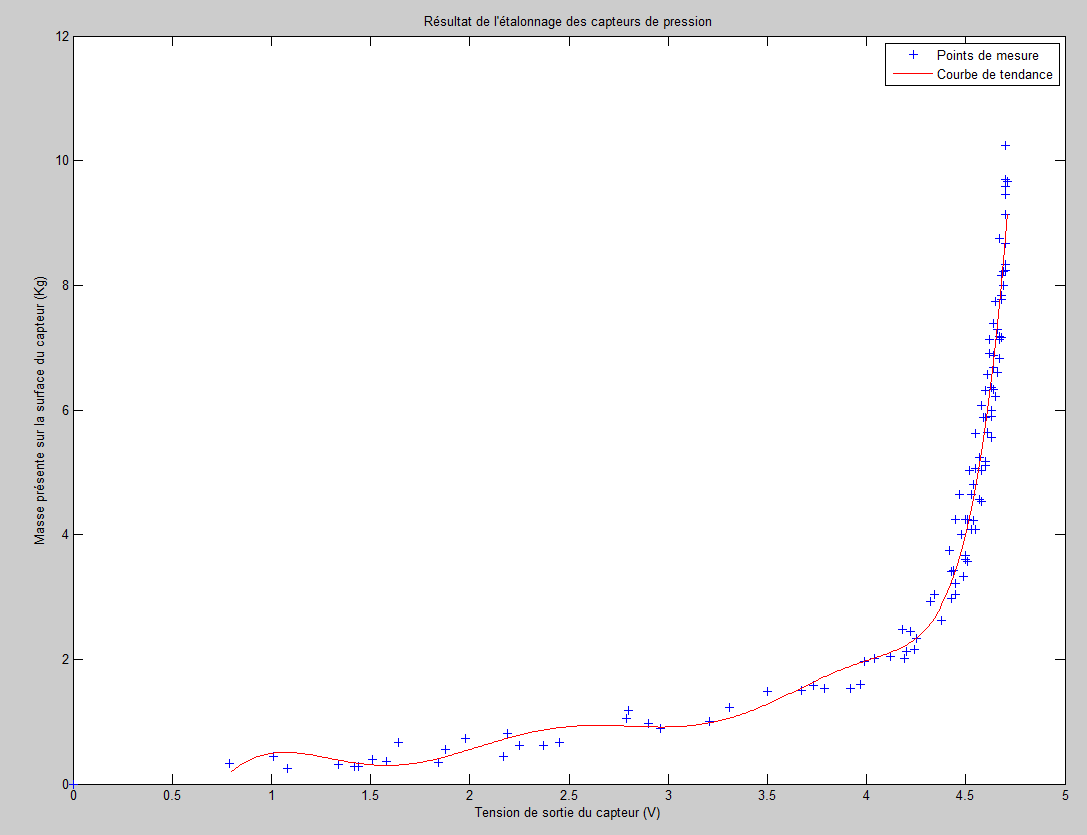
\includegraphics[scale=0.3]{courbe.png}
\caption{\label{fig:courbe} Courbe de tendance obtenue par l"étalonnage des capteurs de pression}
\end{figure} 

Les capteurs de pression se situent au niveau des 4 coins du cadre avec une position très légèrement sur-élevée afin que le matériel reposent uniquement sur ces derniers comme nous pouvons le voir sur la figure \ref{fig:pression2}. Ces capteurs sont positionnés entre 2 plaques rigides en métal afin de limiter les erreurs de mesures. 

\clearpage

\begin{figure}[h!]
\centering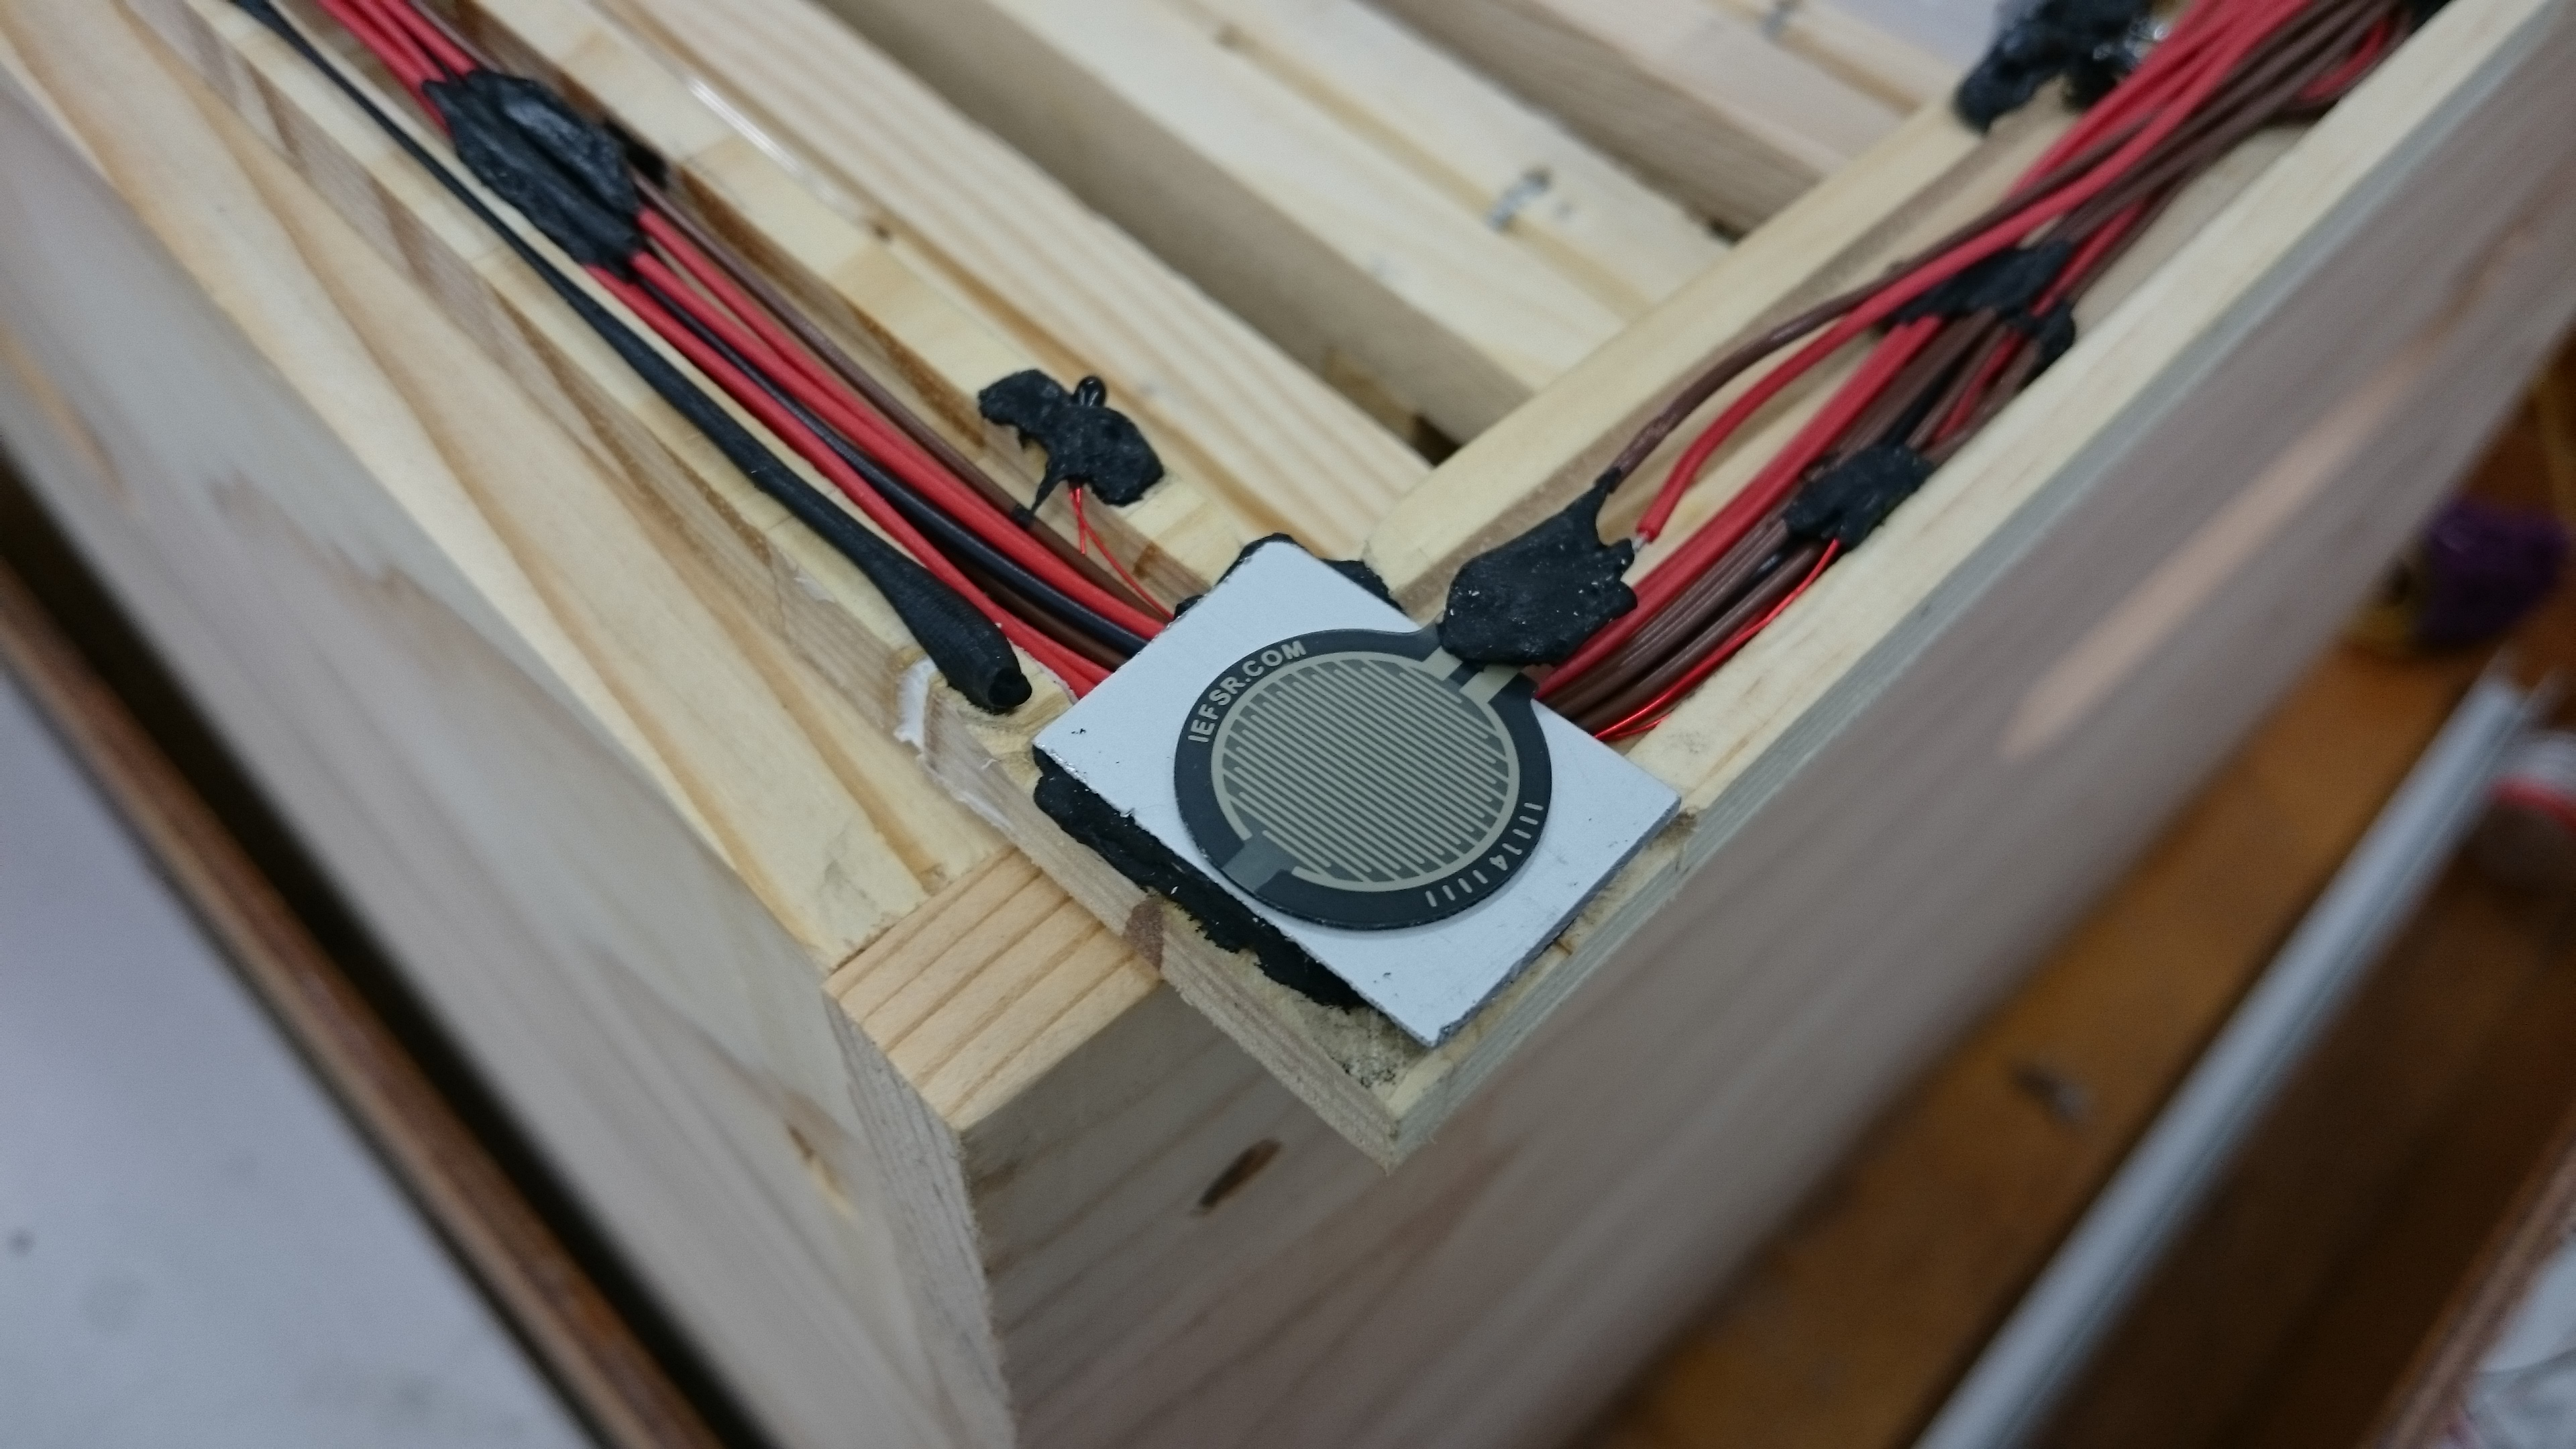
\includegraphics[trim= 0cm 0cm 0cm 0cm,scale=0.08]{pression.jpg}
\caption{\label{fig:pression2} Capteur de pression en position}
\end{figure}

Après avoir installé 2 tilt afin de recueillir le déplacement de la ruche dans 2 directions orthogonales et l'ensemble des autres capteurs (voir figure \ref{fig:cadre2}), nous avons recouvert le cadre avec 4 plaques en métal augmentant ainsi la rigidité. L'isolation a été réalisé grâce à l'emploi d'un mastique placé entre le bois et le métal ainsi qu'à l'intérieur du cadre pour maintenir les fils en place. \\
Une gaine en plastique sera placée à la sortie du cadre pour préserver l'isolation et permettre aux fils de rejoindre la carte où se situent la plaque sur laquelle les 6 thermistances et les 4 capteurs de pression sont placés. Cette plaque, la carte Arduino MEGA 2560, le module GSM/3G de Cooking Hacks et l'antenne seront placés dans un boitier à proximité de la ruche.     

\begin{figure}[h!]
\centering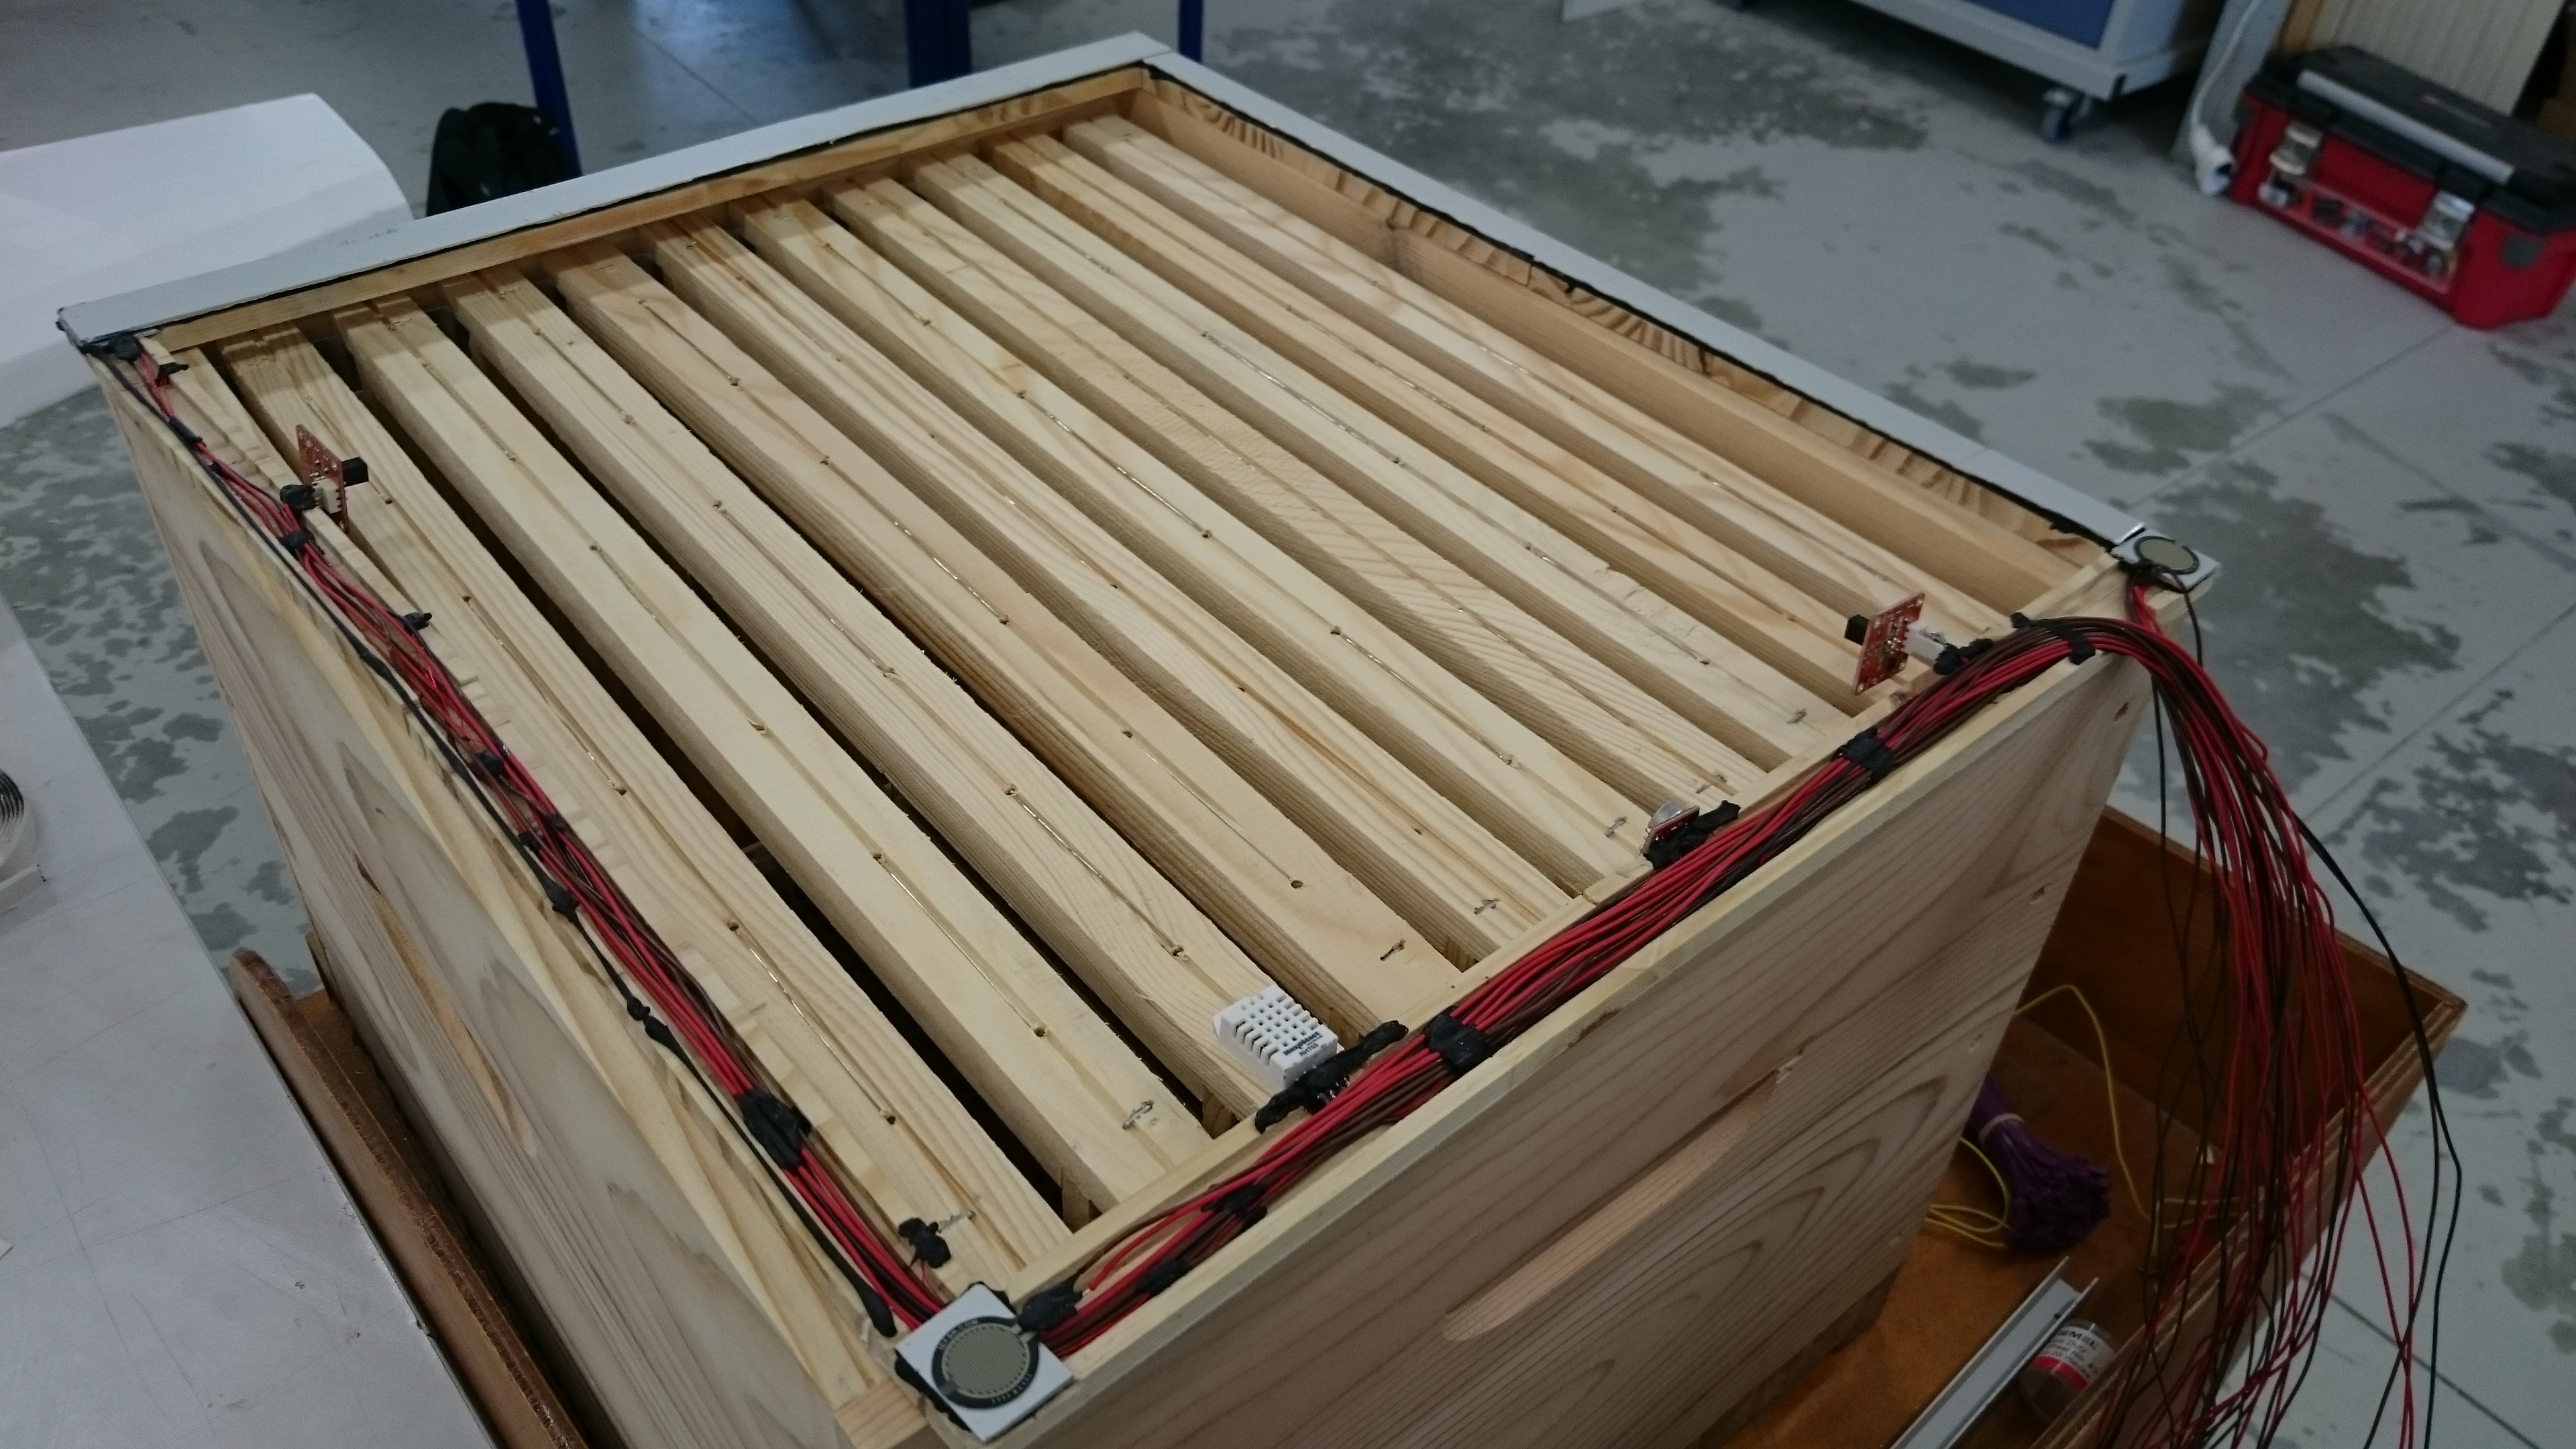
\includegraphics[trim= 0cm 0cm 0cm 0cm,scale=0.08]{cadre2.jpg}
\caption{\label{fig:cadre2} Cadre en cours de montage}
\end{figure}

\clearpage

\section{Gestion des données par Arduino}

Une fois les données recueillis par les capteurs et envoyées vers la carte Arduino, les deux principaux objectifs sont de pouvoir les stocker en local sur une carte SD et de pouvoir les envoyer au serveur pour que l'apiculteur puisse les consulter quelque soit sa position. Pour se faire, nous utiliserons le module GSM/3G de Cooking Hacks de la figure \ref{fig:shield}. Après avoir contacté un grand nombre d'opérateurs téléphonique sur Brest et n'ayant pu obtenir de une carte SIM pour notre projet, nous avons décidé d'utiliser nos propres cartes. 
Le module se programme à l'aide de commande AT (ATtention) qu'il faut exécuter dans un certain ordre en fonction de l'action désirée: envoyer un sms (AT+CPIN=****), établir une connexion HTTP (AT+CHTTPACT=url,port où le port est égal à 80 pour le protocole HTTP)...\\ 
Ces commandes sont spécifique au module que nous utilisons. Dans notre cas, il s'agit d'un SIM 5218 présent sur la figure \ref{shield}.

\begin{figure}[h!]
\centering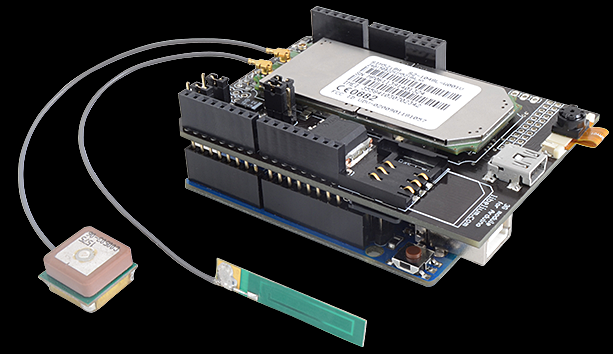
\includegraphics[trim= 0cm 0cm 0cm 0cm,scale=0.50]{shield.png}
\caption{\label{fig:shield} Shield GSM/3G connecté avec une Arduino UNO avec l'antenne de communication et GPS}
\end{figure}

Afin de tester progressivement notre code et comprendre la source des erreurs, nous avons utilisé une carte Arduino UNO en mode Gateway (en retirant le microcontrôleur ATmega) puis en rentrant les commandes AT via le monitor. En effet, il est impossible de retirer me microcontrôleur d'une Arduino MEGA 2560 l'endommager. Le monitor doit être réglé en mode CR-LF (Carriage Return - Line Feed) et choisir une vitesse de transmission de 115200 bauds. Il faut aussi veiller à placer les "jumpers" en position USB et non plus Arduino. Il nous a ensuite fallu télécharger la bibliothèque Time qui permet d'horodater nos mesures lors de leur enregistrement sur la carte SD et pour pouvoir satisfaire le format JSON utilisé par la base de données du serveur.

\clearpage

\begin{figure}[h!]
\centering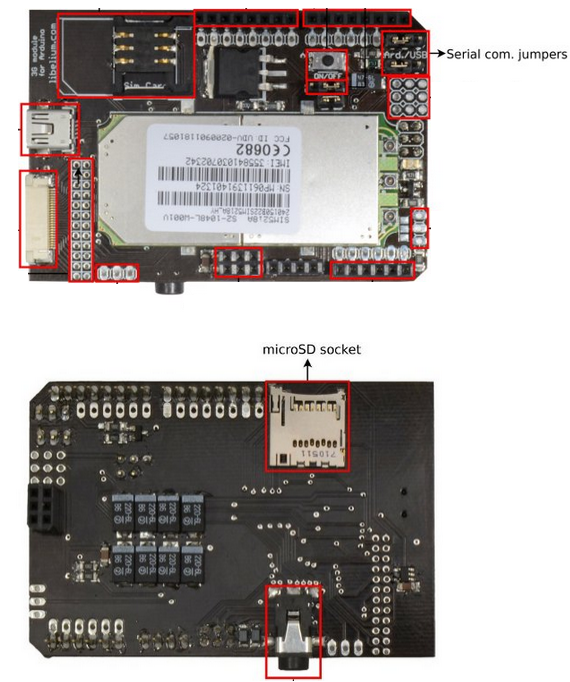
\includegraphics[trim= 0cm 0cm 0cm 0cm,scale=0.50]{jumpers.png}
\caption{\label{fig:jumpers} Vue détaillée du module GSM/3G et de la carte SIM 5218}
\end{figure}

Lorsque nous ne sommes plus en mode Gateway, il faut bien veiller à vérifier/téléverser notre code Arduino avant de connecter le shield GSM/3G. \\
Pour établir une connexion HTTP avec notre module GSM/3G, nous avons utilisé le site http://requestb.in qui permet de créer une URL temporaire que l'on peut utiliser pour effectuer des requêtes GET/POST. On peut alors voir sur ce site si ces requêtes ont bien été reçues. \\
L'alimentation de la carte Arduino sera assurée par des piles. 

\begin{figure}[h!]
\centering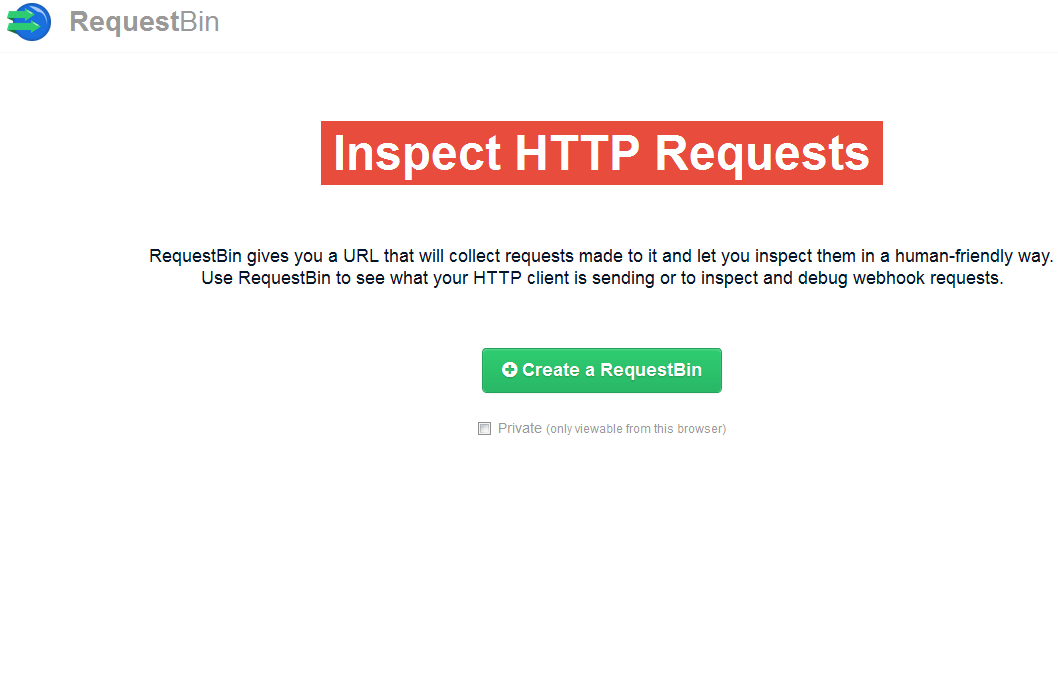
\includegraphics[trim= 0cm 0cm 0cm 0cm,scale=0.45]{requestBin.png}
\caption{\label{fig:requestBin} requestBin}
\end{figure}